\subsection{ART} \label{subsection:android-art}

%
art introduced in kitkat 4.4, available only through developer options,  declared to be preview release, own risk, very little documentation, if any
in lollipop art becomes runtime of choice, supersedes dalvik, breaks compatibility with older dex, as well as itself, very little docu
constantly evolving  through marshmallow, major caveat : oftenc changes in between android minro versions, android optimizes apps everytime you update\newline
art was designed to address shortcomings of dalvik:
virutal machine maintenance is expensie, interpreter/jit simply arent efficient as native code, doing jit all over again on every execution is wasteful, maintenance threads require significantly mroe cpu cycles, cpu cycles translate to slower performance and shorter battery life
dalvik garbage collection frequently causes hangs/jitter
virtual machine architecture is 32bit only, android i sfollowing ios into 64bit space\newline
advantages of art
art mvoes compilation from \gls{jit} to \gls{aot}
VM maintenance not as expensive as dalvik, art compiles to native \gls{aot} not \gls{jit}, less maintenance threads and overhead cycles than dalvik
garbage collection parallizable (foreground/background), non blocking -see- QUELLE
64bit bus some issues still exist -see- quelle\newline
main idea of art/aot:
actually compilation can be to one of two types, quick (native code), portable(llvm code)
in practice preference is to compile to naitve code, portable implies another layer of IR (LLVM's bit code)\newline
Art itself:
art uses not one but two file formats
art - only one file, boot.art, in /syste/framework/architecture (arm,...)
oat - master file, boot.oat, in /syste/framework/architecture (arm,...) - odex files no longer optimized dex but oat, alongeside apk for system apps/frameworks, /data/dalvik-cache for 3rd party apps, still uses odex extension, now file format is elf/oat\newline
art files is a proprietary format, poorly documented, changed format internally repeatedly
art file maps in memory right before oat, which links with it
contains pre-initilited classes, objects and support structures\newline
ART/OAT files are created (on device or on host) by dex2oat
command line saved inside oat file's key value store
\begin{figure}[h]
    \centering
    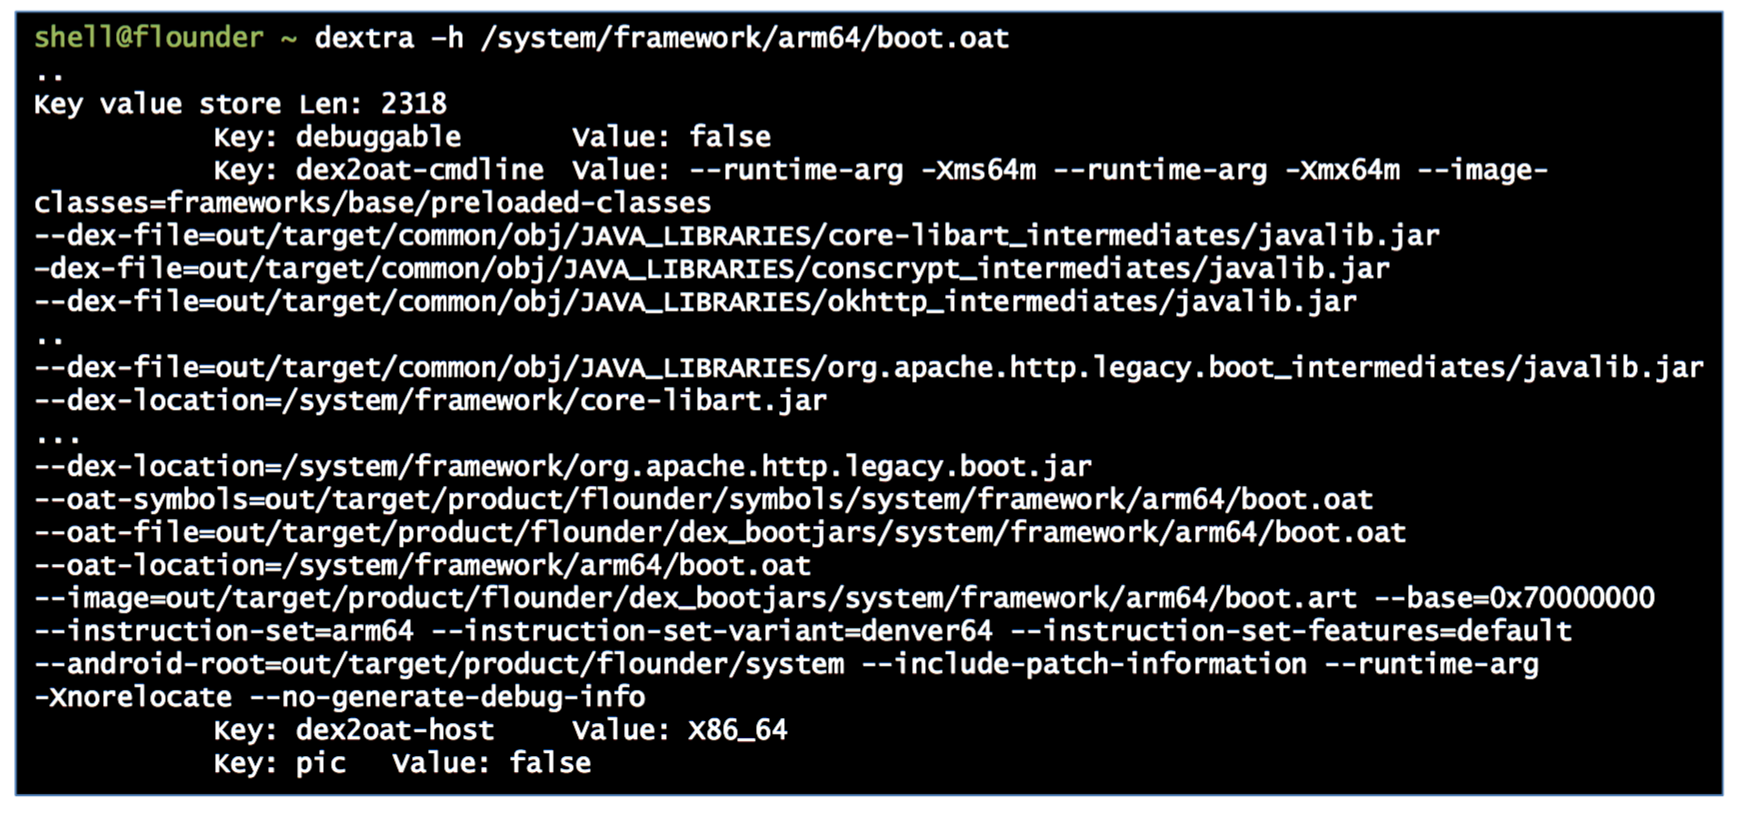
\includegraphics[width=0.8\textwidth]{data/oat.png}
    \caption{Awesome Image}
    \label{fig:awesome_image123}
\end{figure}
\newline
art file format
\begin{figure}[h]
    \centering
    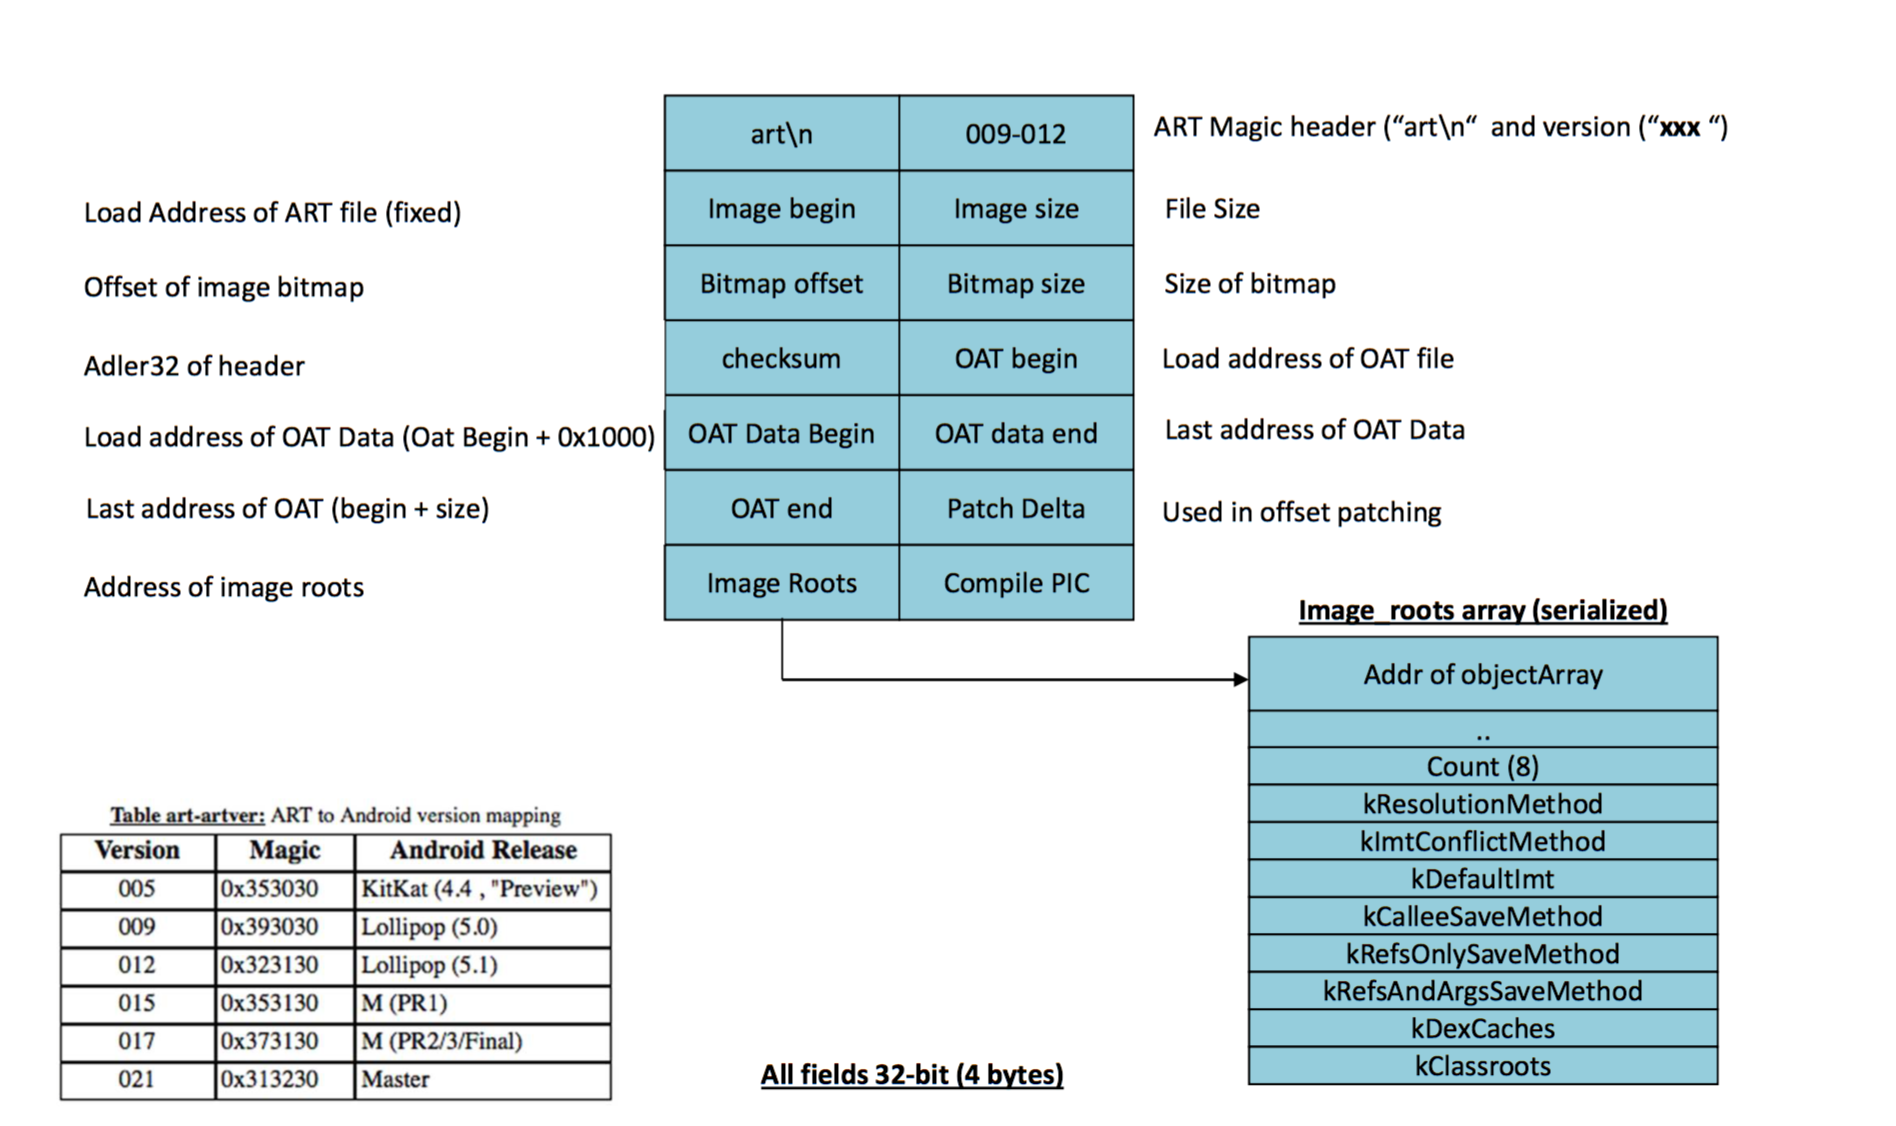
\includegraphics[width=0.8\textwidth]{data/art.png}
    \caption{Awesome Image}
    \label{fig:awesome_image1223}
\end{figure}
\begin{figure}[h]
    \centering
    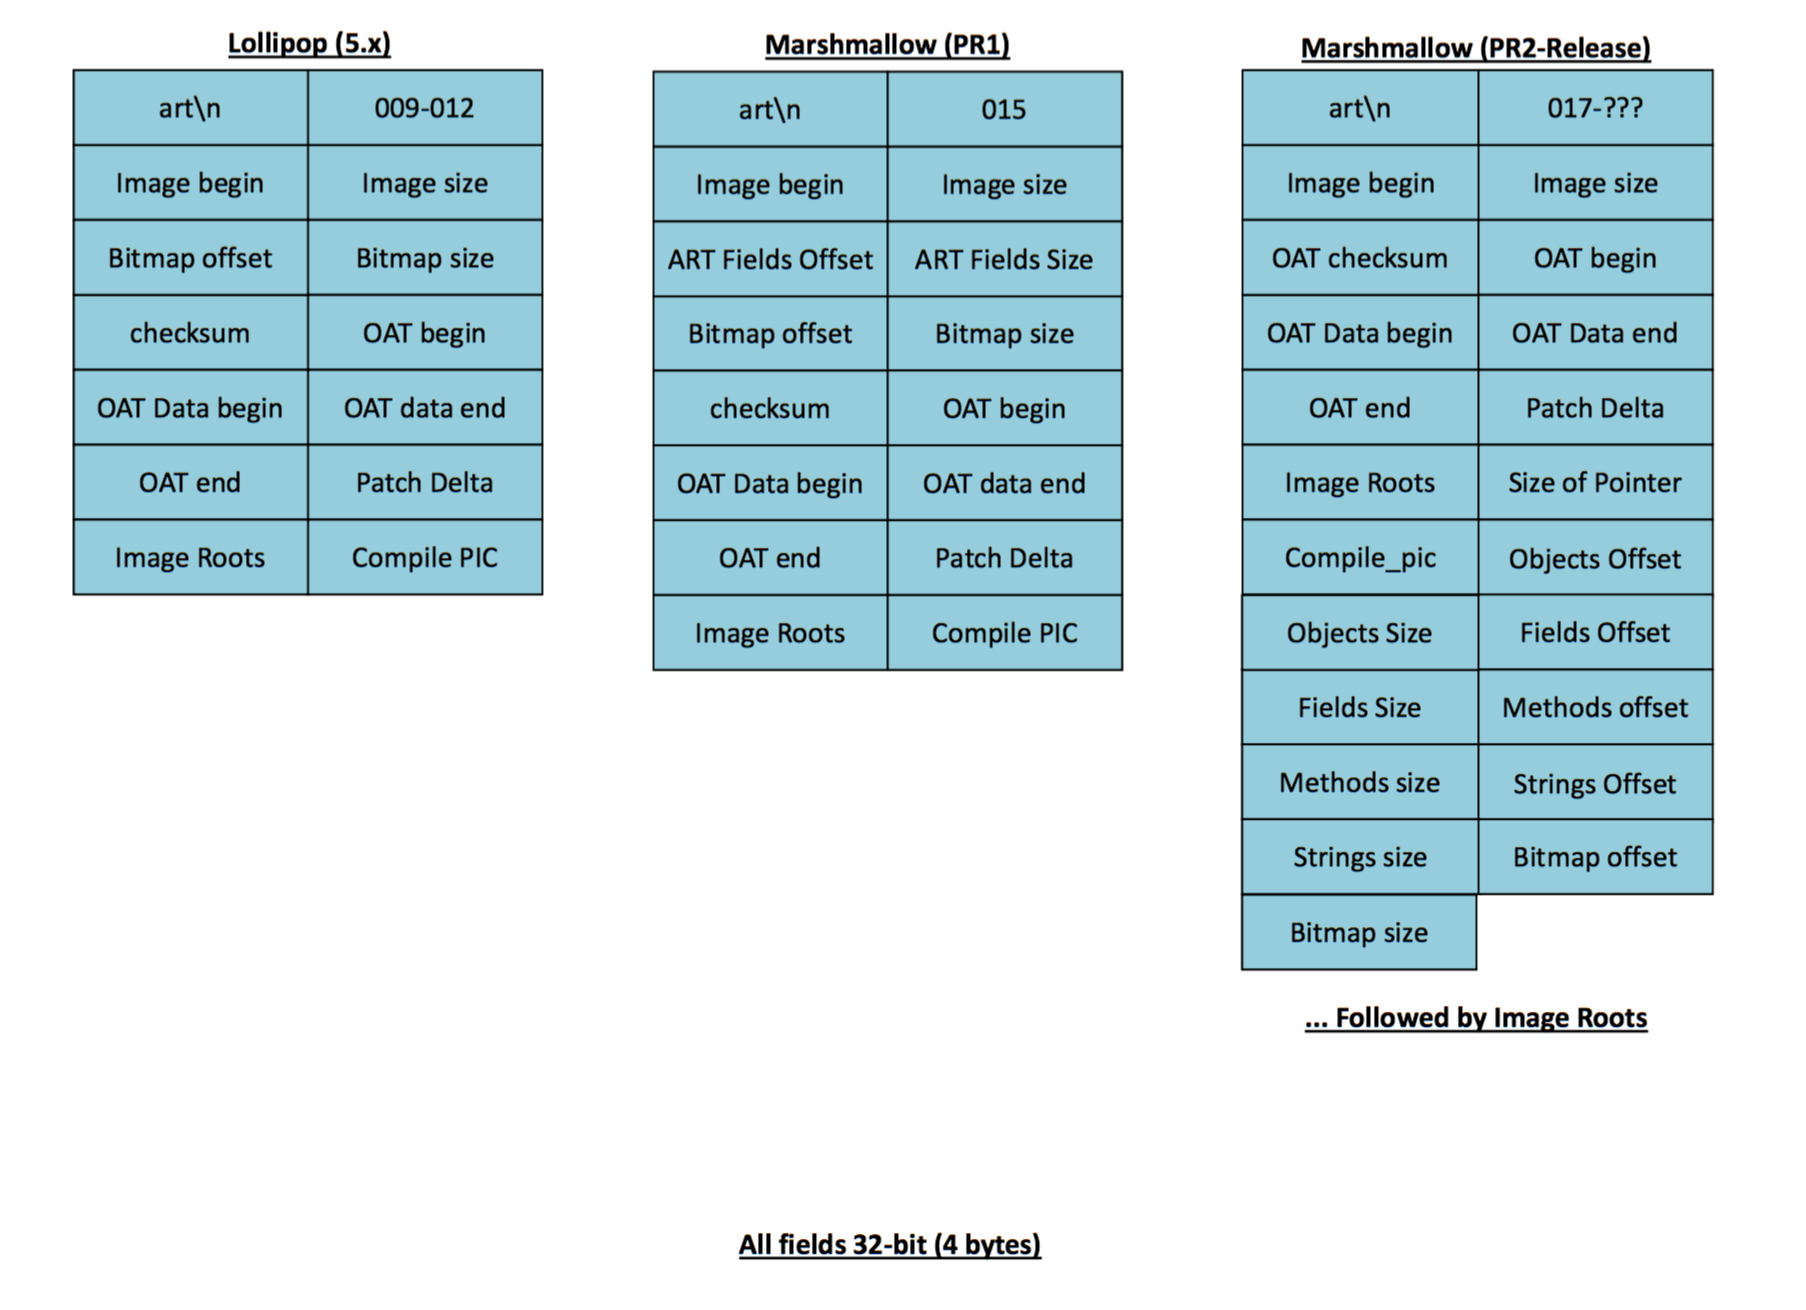
\includegraphics[width=0.8\textwidth]{data/art2.png}
    \caption{Awesome Image}
    \label{fig:awesome_image12223}
\end{figure}
\newline

OAT and ELF
oat are actully embedded in ELF object files (was ist elf?)
\begin{figure}[h]
    \centering
    \includegraphics[width=0.8\textwidth]{data/elf.png}
    \caption{Awesome Image}
    \label{fig:awesome_image12223}
\end{figure}

\newline
the oat dexfile header
oat headers are 1...n dex files, actual value given by dexfilecount field in header
\begin{figure}[h]
    \centering
    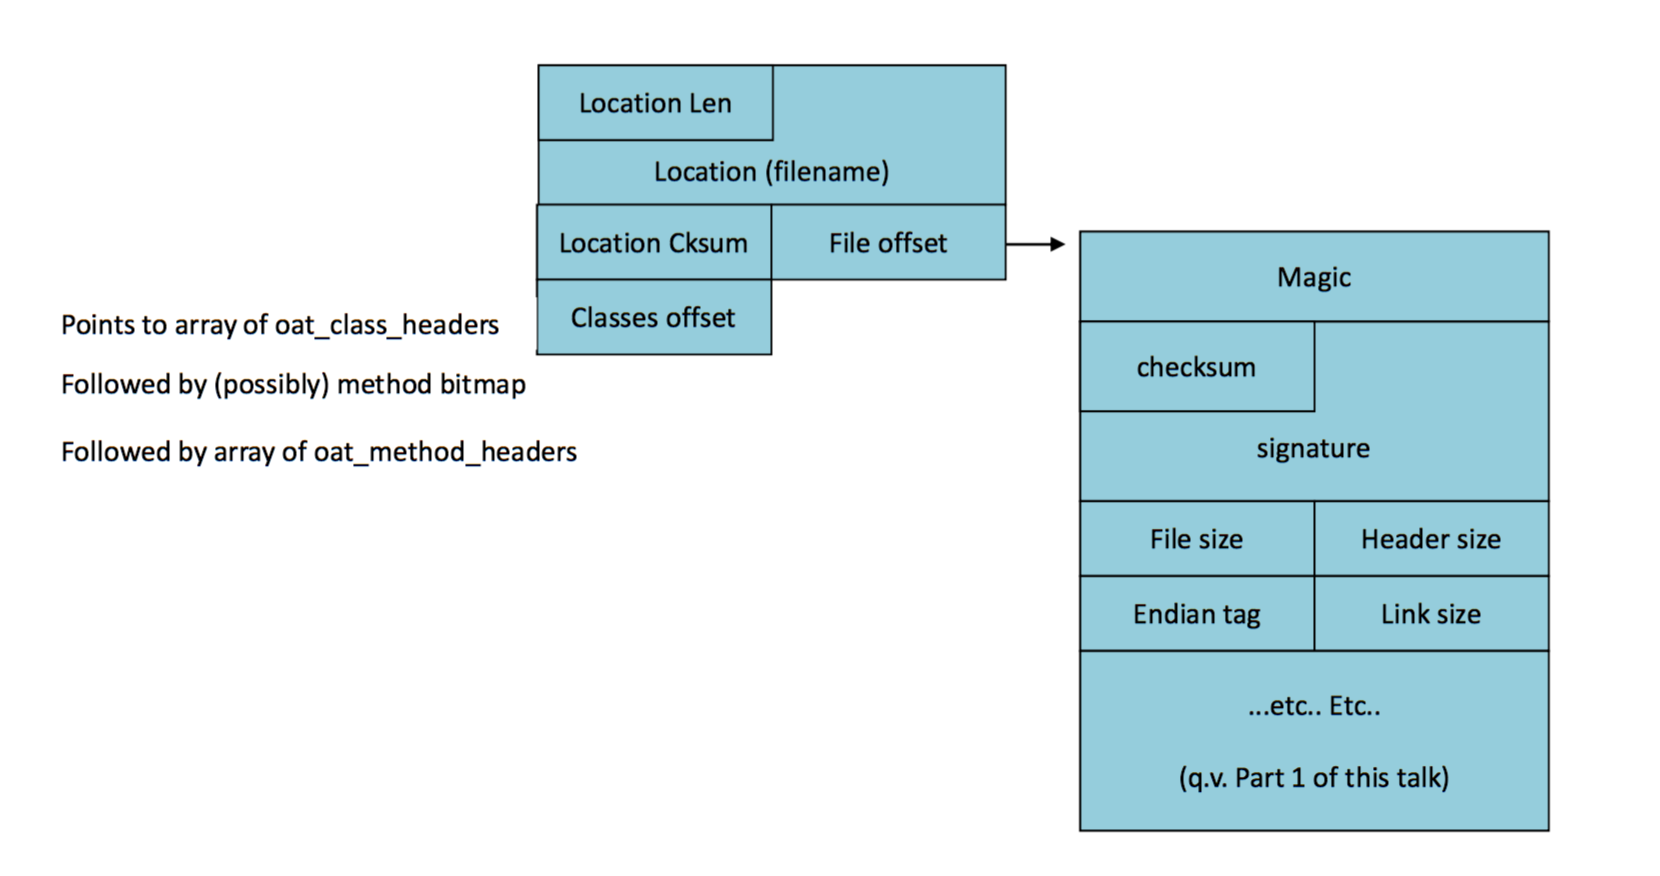
\includegraphics[width=0.8\textwidth]{data/oatdex.png}
    \caption{Awesome Image}
    \label{fig:awesome_image122223}
\end{figure}

\newline
finding dex in oat
odex files will usually have only one (=original) dex embedded
booat.oat is something else entirely, some 14 dex files the best of the android framework jars, each dex contains potentilly hundres of classes

\newline
art code generation
oat method headers point to offset of native code
each method has a quick or portable method header, contains mapping from virtual register to underlying machine registers
each method has a quick or protable frame info, provides frame size in bytes, core register spill mask, fp register spill mask
generated code uses unusual registers, especially fond of using lr as call register, still saves/restores registers so as not to violate arm conventions
\newline
art supports mutliple architectures(x86,arm/64,mips)
compiler is layered architecture, using portable (llvm) adds another lvl with llvm bitcode (not in this scope)
\begin{figure}[h]
    \centering
    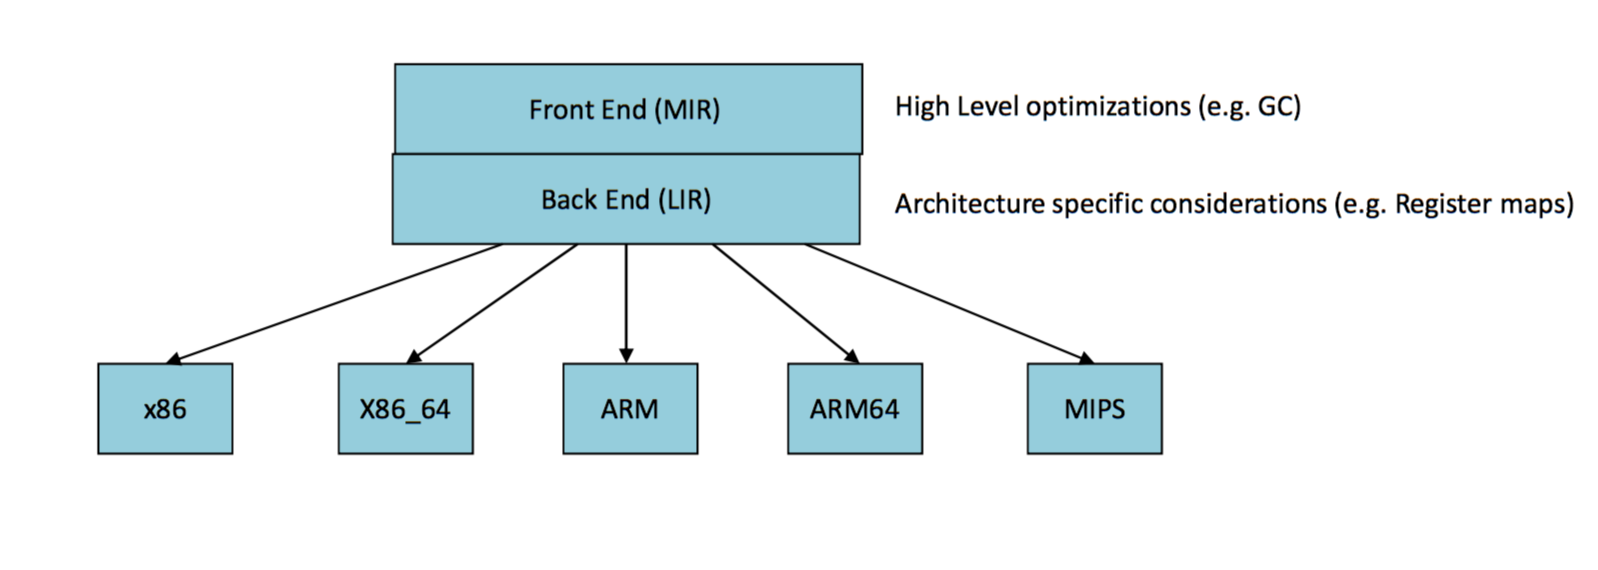
\includegraphics[width=0.8\textwidth]{data/artarch.png}
    \caption{Awesome Image}
    \label{fig:awesome_image122223}
\end{figure}
\newline

vergleich java/dex/odex(art) code
\newline

lessons
base code is dex so vm is still 32bit, no 64bit registers or operands so mapping to underlying arch inst always 64bit, there are actually a frw 64bit instructions but most dex code doesnt use them
generated code isnt always that efficient, not on same par as an optimizing antive code compiler, likely to improve with llvm optimizations
overall code (determined by Mir optimizations) flow is same
garbage collection, register maps, likewase same
cavears: not all methods guaranteed to be compiled, reversing can be quite a pain
\newline

ART runtime threads
the daemon threads are started in java by libcore, daemon class wraps thread class and provides singleton INSTANCE, do same basic operations as they did in "classic" dalvikVM, libart subree in libcore implementation slightly different
\newline

isn't android all dalvik now?
art is runtime but application compile into dex, art is compiled on device during install, art binaries has dalvik embedded, some methods may be left as dex to be interpreted, dalvik is miuch easier to debug than art --see- evaluation \newline
\cite{andevconDalvikART}
%
